\documentclass[a4paper,11pt]{article}
\usepackage{amsmath,amsthm,amsfonts,amssymb,amscd,amstext,vmargin,graphics,graphicx,tabularx,multicol} \usepackage[french]{babel}
\usepackage[utf8]{inputenc}  
\usepackage[T1]{fontenc} 
\usepackage[T1]{fontenc}
\usepackage{amsmath,amssymb}
\usepackage{pstricks-add,tikz,tkz-tab,variations}
\usepackage[autolanguage,np]{numprint} 
\usepackage{color}
\usepackage{ulem}

\setmarginsrb{1.5cm}{0.5cm}{1cm}{0.5cm}{0cm}{0cm}{0cm}{0cm} %Gauche, haut, droite, haut
\newcounter{numexo}
\newcommand{\exo}[1]{\stepcounter{numexo}\noindent{\bf Exercice~\thenumexo} : \marginpar{\hfill /#1}}
\reversemarginpar


\newcounter{enumtabi}
\newcounter{enumtaba}
\newcommand{\q}{\stepcounter{enumtabi} \theenumtabi)  }
\newcommand{\qa}{\stepcounter{enumtaba} (\alph{enumtaba}) }
\newcommand{\initq}{\setcounter{enumtabi}{0}}
\newcommand{\initqa}{\setcounter{enumtaba}{0}}

\newcommand{\be}{\begin{enumerate}}
\newcommand{\ee}{\end{enumerate}}
\newcommand{\bi}{\begin{itemize}}
\newcommand{\ei}{\end{itemize}}
\newcommand{\bp}{\begin{pspicture*}}
\newcommand{\ep}{\end{pspicture*}}
\newcommand{\bt}{\begin{tabular}}
\newcommand{\et}{\end{tabular}}
\renewcommand{\tabularxcolumn}[1]{>{\centering}m{#1}} %(colonne m{} centrée, au lieu de p par défault) 
\newcommand{\tnl}{\tabularnewline}

\newcommand{\trait}{\noindent \rule{\linewidth}{0.2mm}}
\newcommand{\hs}[1]{\hspace{#1}}
\newcommand{\vs}[1]{\vspace{#1}}

\newcommand{\N}{\mathbb{N}}
\newcommand{\Z}{\mathbb{Z}}
\newcommand{\R}{\mathbb{R}}
\newcommand{\C}{\mathbb{C}}
\newcommand{\Dcal}{\mathcal{D}}
\newcommand{\Ccal}{\mathcal{C}}
\newcommand{\mc}{\mathcal}

\newcommand{\vect}[1]{\overrightarrow{#1}}
\newcommand{\ds}{\displaystyle}
\newcommand{\eq}{\quad \Leftrightarrow \quad}
\newcommand{\vecti}{\vec{\imath}}
\newcommand{\vectj}{\vec{\jmath}}
\newcommand{\Oij}{(O;\vec{\imath}, \vec{\jmath})}
\newcommand{\OIJ}{(O;I,J)}

\newcommand{\bmul}[1]{\begin{multicols}{#1}}
\newcommand{\emul}{\end{multicols}}


\newcommand{\reponse}[1][1]{%
\multido{}{#1}{\makebox[\linewidth]{\rule[0pt]{0pt}{20pt}\dotfill}
}}

\newcommand{\titre}[5] 
% #1: titre #2: haut gauche #3: bas gauche #4: haut droite #5: bas droite
{
\noindent #2 \hfill #4 \\
#3 \hfill #5

\vspace{-1.6cm}

\begin{center}\rule{6cm}{0.5mm}\end{center}
\vspace{0.2cm}
\begin{center}{\large{\textbf{#1}}}\end{center}
\begin{center}\rule{6cm}{0.5mm}\end{center}
}



\begin{document}
\pagestyle{empty}
\titre{Interrogation : Notions de fonctions}{Nom :}{Prénom :}{Date}{Classe}

\vspace*{0.5cm}

\exo{2} Soit $f$ une fonction définie par le graphique ci-dessous.

\bmul{2}

\includegraphics[scale=0.95]{interrograph.eps} 


\columnbreak


\initq \q Lire graphiquement l'image par la fonction $f$ de :\\
\hspace*{0.5cm} \qa 2 ? \hspace*{0.5cm} \qa 8 ?  \\
\reponse[4]\\

 

\emul

\q Lire graphiquement le ou les antécédents par la fonction $f$ de :\\
 \initqa
\hspace*{0.5cm} \qa 3 ?  \hspace*{0.5cm} \qa 1 ?\\
\reponse[4]\\

\vspace*{0.75cm}






\exo{2.5} Voici un tableau de valeur d'une fonction $h$.\\

\includegraphics[scale=0.65]{interrograph2.eps} \\

\initq \q Compléter les inégalités suivantes : \hspace*{0.5cm} $h$(. . . ) = -2 \hspace*{0.75cm} $h(1,5)=$ . . .   \\

\q Donner le ou les antécédents de -1,5 par la fonction $h$.\\
\reponse[2]\\

\q Quelle est l'image de -0,5 par la fonction $h$ ?\\
\reponse[1]\\

\newpage

\vspace*{0.25cm}

\exo{2.5} Soit $g$ la fonction définie par $g(x) = 7x-9$. \\

\initqa
\qa Calculer $g(2,5)$.\\
\reponse[3]\\

\qa Calculer l'image de $\dfrac{1}{3}$ par la fonction $g$.\\
\reponse[3]\\

\qa Calculer l'antécédent de 12.\\
\reponse[4]\\

\vspace*{0.25cm}

\exo{3} Soit $f$ la fonction définie par $f(x) = -3x^{2}+2x-5$. \\


\initq
\q Quelle est l'image de 2 par la fonction $f$? \\
\reponse[5]\\

\q Quelle est l'image de -1 par la fonction $f$?\\
\reponse[5]\\

\exo{}BONUS \hspace*{0.5cm}
Deux trains partent ensemble à 10h12 : le premier part de
Paris pour rejoindre Strasbourg, le second part de Strasbourg pour rejoindre Paris.\\
 Ils roulent sur la même ligne,
le premier à une vitesse moyenne de 220 km/h et le second à 180 km/h.\\
Lequel sera le plus près de Paris quand ils se croiseront?\\
\reponse[4]




\end{document}
